\documentclass{sig-alternate}
\usepackage{textcomp}
\usepackage{graphics}
\pagestyle{plain}
\usepackage{subfigure}
\usepackage[margin=10pt,font=small,labelfont=bf, labelsep=endash, skip=0pt]{caption}
\usepackage[latin1]{inputenc}
\usepackage{listings}

\begin{document}

\pagenumbering{arabic}

\title{Mahjong Solitaire}
\subtitle{Sistemas de Inteligencia Artifical - ITBA}

\numberofauthors{3}

\author{
	\alignauthor{Carlos Sessa}\\
	\alignauthor{Lucas Pizzagalli}\\
	\alignauthor{Nicol\'as Purita}\\
}

\date{09 de Mayo de 2011}

\maketitle

\section*{Introducci\'on}
	Se implementa un \textit{Sistema de Producci\'on} el cual es utilizado para resolver un juego denominado \textbf{Mahjong-Solitaire}, tambien conocido como el \textit{Taipei}. Se utiliza un motor de inferencia en \textit{Java} para la resoluci\'on del problema designado, el cual fue entregado por la c\'atedra. \\
	Como punto de partida para crear el \textit{Sistema de Producci\'on} se dise\~{n}a un sistema de almacenamiento apropiado que represente el problema de la forma m\'as \'optima. Se utilizan 3 estrat\'egias de b\'usqueda no informadas para comparar las distintas soluciones alcanzadas, las cuales se detallan en el transcurso del informe.

\section*{Reglas del Mahjong-Solitaire}
	El juego \textbf{Mahjong-Solitaire} consiste en eliminar todas las fichas de un tablero de 144 fichas. \\
	Una ficha puede ser removida siempre que no se encuentre bloqueada y ademas cumpla con la condici\'on de que las fichas son del mismo tipo. Las fichas existentes son:

\begin{table}[h]
\begin{center}
	\begin{tabular}{|c|c|c|}
	\hline
	 Tipo de Ficha & Identificador & Cantidad\\
	\hline \hline
	\textit{Character} & 9 & 4 de c$\setminus$u \\
	\textit{Bamboo} & 9 & 4 de  c$\setminus$u  \\
	\textit{Circles} & 9 & 4 de  c$\setminus$u  \\
	\textit{Dragons} & 3 & 4 de  c$\setminus$u  \\	
	\textit{Winds} & 4 & 4 de  c$\setminus$u  \\
	\textit{Season} & 4 & 1 de c$\setminus$u \\
	\textit{Flowers} & 4 & 1 de  c$\setminus$u  \\
	\hline
	\end{tabular}
\end{center}
\caption{Distribuci\'on de fichas}
\label{tab:tiles}
\end{table}

	Existe una excepci\'on en la remoci\'on de las fichas del tipo \textit{Season} o \textit{Flowers}. La excepci\'on esta basada en que cualquier ficha de \textit{Season} o \textit{Flowers} puede ser removida en conjunto con otra del mismo grupo por más que no sea igual. Ejemplo: Summer con Winter. \\
	Una ficha bloqueada puede estar en forma \textit{Horizontal}, \textit{Vertical} o \textit{Ambos}. Estos bloqueos se definen del siguiente modo:
	\begin{itemize}
		\item \textbf{Horizontal}: La ficha elegida posee una ficha a su izquierda y derecha.
		\item \textbf{Vertical}: La ficha elegida posee una ficha encima de ella.		
	\end{itemize}
	En la Figura \ref{fig:blocking} se puede observar distintas posibilidades de bloqueos.
\section*{Desarrollo}

	Se representa un estado del juego como un vector de vectores en donde cada celda posee una \textit{Tile}. Este vector de vectores es del tipo:
	\begin{itemize}
		\item \textit{Tile}[a][b][c]
	\end{itemize}
	donde \textit{a} indica el nivel en el que se encuentra la ficha, \textit{b} es la fila y \textit{c} la columna. La clase \textit{Tile} est\'a definida como la composici\'on de un tipo de ficha y un n\'umero.
	
\section*{Funciones de costo}

	Dado que el objetivo del juego es simplemente retirar todas las fichas del tablero, la funci\'on de costo propuesta es la cantidad de fichas sacadas en cada estado, la cual se denomina \textit{$g_1$}. \\
	Se debe notar que si las reglas s\'olo sacan fichas de a pares, la funci\'on de costo es constante. Caso contrario, si alguna regla saca m\'as de un par, la funci\'on de costo es variable.

\section*{Heur\'isticas}

	Se considera \textit{Pair} a todo par de fichas posibles a retirar del tablero en un estado y \textit{Payers} a la lista de \textit{Pares} que pueden retirarse del tablero. \\
	Se proponen las siguientes heur\'isticas (para desarrollar en las estrat\'egias de b\'usquedas no informadas):
	\begin{itemize}

		\item \textbf{M\'as Alta} \textit{(h1)}: Se libera el \textit{Pair} de m\'as alto nivel. En el mejor de los casos la remoci\'on de una ficha en una capa m\'as alta puede liberar cuatro fichas, lo cual aumenta la cantidad de \textbf{Payers} en la siguiente jugada.
		
		\item \textbf{Mayor cantidad de fichas horizontales} \textit{(h2)}: Esta heur\'istica busca reducir la posibilidad de eliminar una fila del tablero. La heur\'istica se basa en calcular la cantidad de fichas que posee cada una del \textit{Pair} en la fila en la que se encuentra, esto se calcula como:
			\begin{eqnarray}
				X_{1}  & = & \# Fichas_{izq}+ \# Fichas_{der} \\
				X_{2}  & = & \# Fichas_{izq}+ \# Fichas_{der} \\
				\textbf{h2} & = & X_{1} + X{2}
			\end{eqnarray}
		donde $X_{1}$ y $X_{2}$ es un \textit{Pair}. Esta heur\'istica se basa en reducir la posibilidad de eliminar las filas que se encuentran en los niveles mas bajos, debido a que no liberan nuevos \textit{Payers}.
		
		\item \textbf{Generador M\'aximo de \textit{Payers}} \textit{(h3)}: Esta heur\'isitca se basa en eliminar los \textit{Pairs} que generen mayor cantidad de \textit{Payers} en el pr\'oximo estado.
		
	\end{itemize}

\section*{Resultados y Conclusiones}	
En la tabla \ref{tab:cost} se ven los distintos resultados para distintas estrategias de b\'usqueda	 en algoritmos no informados. \\
Se ve que para la estrategia \emph{DFS} se logran mejores resultados que para \emph{BFS} y \emph{Profundizaci\'on iterativa}, en el sentido del tiempo promedio y nodos expandidos, dado que todos llegan a la soluci\'on en un tablero de nivel f\'acil ya que en tableros mas complejos (con 144 fichas) no se alcanza una soluci\'on. Esto se debe a que todas las posibles soluciones del problema se encuentran a la misma altura. Mientras que \emph{BFS} y \emph{Profundizaci\'on Iterativa} explotan nodos donde no est\'a la soluci\'on, DFS alcanza m\'as r\'apido las hojas. Dada la naturaleza del problema, no existen soluciones sub\'optimas, por lo tanto si se encuentra una soluci\'on, sabemos que es la mejor.\\
 Es por eso que si \emph{DFS} entra en la rama de la soluc\'ion, seguro llega a esta y no expande m\'as nodos. En cambio, \emph{BFS} no encontrar\'a la soluci\'on hasta explorar el \'ultimo nivel y lo mismo sucede con \emph{Profundizaci\'on iterativa}. \\
En los tableros \ref{fig:layout3} y \ref{fig:layout4} utilizando \emph{BFS} y \emph{Profundizaci\'on Iteratica} se observa que es necesario expandir todo el \'arbol, por lo que en un tiempo aproximado de 5 minutos no se puede llegar a la soluci\'on. De todos modos se realizaron pruebas con \'ordenes de magnitud mas grandes a este tiempo (7 horas y 30 minutos aprox.) y se concluy\'o a que \emph{BFS} no termina ya que debe expandir hasta el \'ultimo nivel para obtener una soluci\'on.

\onecolumn

\begin{figure}[h!]
  \begin{center}
  	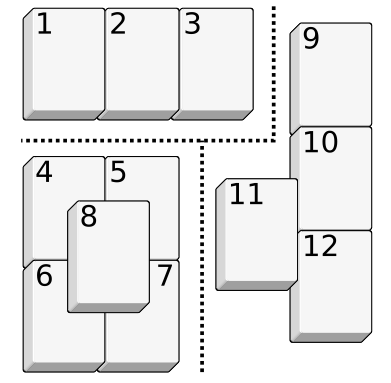
\includegraphics[scale=0.3]{images/blocking.png}
  \end{center}
  \caption{Ficha 2 es bloqueada por la 1 y 3. La ficha 4-7 est\'an bloqueadas por la 8. El resto de las fichas son movibles.}
  \label{fig:blocking}
\end{figure}

\begin{figure}[h!]
  \begin{center}
      \subfigure[Tablero 1]{\label{fig:layout1}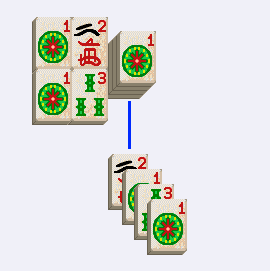
\includegraphics[scale=0.3]{Boards/Layout1.png}}
    \hspace{20pt}
    \subfigure[Tablero 2]{\label{fig:layout3}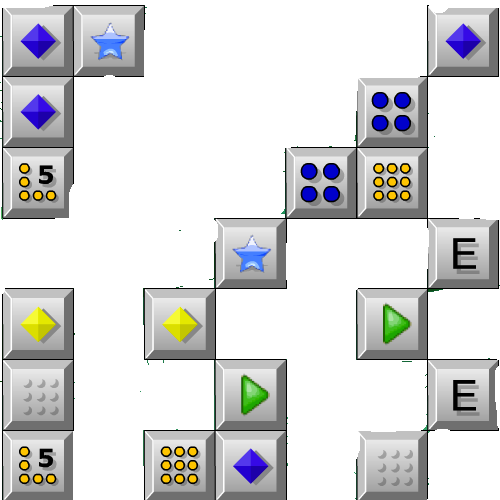
\includegraphics[scale=0.2]{Boards/Layout3.png}}
    \hspace{20pt}
    \subfigure[Tablero 3]{\label{fig:layout4}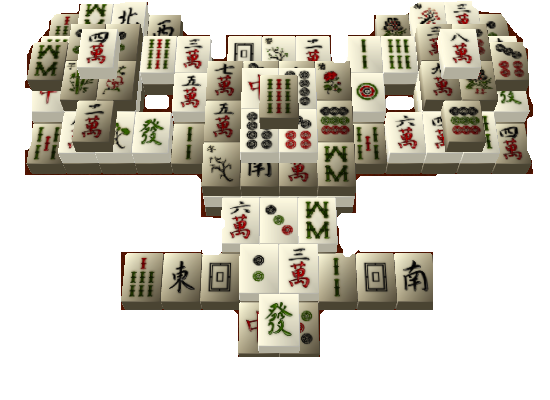
\includegraphics[scale=0.2]{Boards/Layout4White.png}}
  \end{center}
  \caption{Distintos tableros}
  \label{fig:layouts}
\end{figure}
	
	
\begin{table}[h]
\begin{center}
	\begin{tabular}{|p{2.3cm}|p{2cm}|p{2cm}|p{2cm}|p{2cm}|p{4cm}|}
	\hline
	 Algoritmo & Nodos expandidos & Nodos en la frontera & Nodos generados & Profundidad de la Soluci\'on & Tiempo de Procesamiento\\
	\hline \hline
		 \multicolumn{6}{|c|}{Layout 1} \\
	\hline
	\textit{DFS} & 6 & 0 & 6 & 4 & 32ms \\
	\textit{BFS} & 7 & 0 & 6 & 4 & 10ms \\
	\textit{Produndizaci\'on Iterativa} & 7 & 7 & 19 & 4 & 12ms \\
	\hline
		 \multicolumn{6}{|c|}{Layout 2} \\
	\hline
	\textit{DFS} & 11 & 57 & 10 & 10 & 74ms \\
	\textit{BFS} &5944 & 34491 & 5944 & ? & 5' \\
	\textit{Produndizaci\'on Iterativa} & 7550 & 33571 & 5696 & ? & 5' \\
	\hline
		 \multicolumn{6}{|c|}{Layout 3} \\
	\hline
	\textit{DFS} & 73 & 1438 & 72 & 72 & 2' 708ms \\
	\textit{BFS} & 641 & 15705 & 641 & ? & 5' \\
	\textit{Produndizaci\'on Iterativa} & 620 & 14964 & 587 & ? & 5' \\
	\hline
	\end{tabular}
\end{center}
\caption{Resultados de resolver el problema de los tableros \ref{fig:layout1}, \ref{fig:layout3} y \ref{fig:layout4} con distintos algoritmos no informados}
\label{tab:cost}
\end{table}

\end{document}